%%%%%%%%%%%%%%%%%%
\section{Herramienta TPTVPH}
\label{rasim:posing}

La \emph{suite} \ac{ITGVPH} se encargará de generar la base de datos necesaria para que los usuarios puedan entrenar con una variabilidad anatómica extensa. Esto permite al usuario enfrentarse a diferentes tipos de situaciones y mejorar el entrenamiento del procedimiento. En ocasiones el procedimiento médico que se va a realizar necesita que los modelos virtuales disponibles se encuentren en una posición diferente a la postura que presentan. Por lo tanto, surge la necesidad de incluir un algoritmo que adapte un paciente virtual.

%
%Para modificar esa postura, se necesitaría un algoritmo que sea capaz de transformar un modelo virtual con estructuras internas de una pose a otra. Debido que en la mayoría de las ocasiones, no se dispone de todos los tejidos o de sus propiedades mecánicas, este método deberá ser capaz de generar deformaciones plausibles útiles para el entrenamiento.


%La tarea 3.5 del \del{ac{WP} 3} define el requisito de que la herramienta \ac{ITGVPH} permita adaptar la posición del paciente virtual creado de una postura inicial a la requerida por el simulador \ac{RASim}. 
Para ello,  se va a incorporar el algoritmo propuesto, descrito en el capítulo \ref{cap:posing}, a una aplicación llamada \ac{TPTVPH}. Esta herramienta se ha construido para proporcionar una interfaz donde el usuario pueda seleccionar la postura del paciente virtual. De esta forma, un usuario con perfil sanitario podrá seleccionar y validar las posiciones que sean requeridas en el procedimiento médico que se desee simular.



%Para ello, se ha habilitado una ventana utilizando la librería \emph{OpenGL}\ref{adsf} y \emph{Qt}\ref{asdf}\todo{revisar} permitiendo al usuario pueda manipular el modelo anatómico desde todas las posiciones que necesite.
Como primer paso, se ha dotado a la interfaz de una ventana donde el usuario puede observar el modelo anatómico. Con el objetivo de poder confirmar las correctas deformaciones del paciente virtual, el usuario puede interaccionar con la escena, de esta forma, y de manera intuitiva puede utilizar el ratón para mover, rotar, acercar o alejar el modelo y poder supervisar la deformación desde todos los ángulos posibles.

En segundo lugar, para permitir la selección de poses, se han incluido en la interfaz botones y actuadores, que permiten al usuario seleccionar las articulaciones del \ac{VPH} una a una y definir sus movimientos respecto a los centros de rotaciones calculados (ver sec. \ref{posing:rigging}). El usuario puede revisar poses anteriormente almacenadas, modificarlas y guardarlas de nuevo. También, con el objetivo de introducir movimientos más orgánicos, el sistema permite cargar animaciones provenientes de \ac{MoCap}, o utilizar la tecnología del dispositivo \emph{Microsoft Kinect} en forma de espejo para definir la postura del \ac{VPH} (ver sec. \ref{posing:Poses}).

Además, se ha incorporado una funcionalidad que permite al usuario decidir si quiere esconder tejidos con la finalidad de contemplar la anatomía interna que estuviera oculta. De esta manera, se permite dejar de \emph{renderizar} la piel o los músculos para contemplar otros órganos.% más profundos. 

Finalmente, se ha delegado la responsabilidad de generar posiciones correctas o realistas al usuario. En la sección \ref{posing:optimizacion}, se presenta una etapa optimización que se apoya en un modelo basado en física para mejorar el resultado obtenido. Al ser una etapa no interactiva, solo se activa cuando el usuario decide utilizarla. Una vez terminado el proceso, se podrá observar los resultados y almacenar el paciente virtual obtenido que será utilizado en las demás etapas de la \emph{suite} \ac{ITGVPH}.  

%Por último,  ha sido necesaria la adaptación del sistema para poder adecuarse a los formatos de fichero de entrada y salida de los modelos anatómicos. El formato elegido es \ac{X3D} de manera que será utilizados tanto por la herramienta \ac{ITGVPH} como por el simulador \ac{RASim}.

%\subsection{Interfaz de usuario \ac{TPTVPH}}
\paragraph{Interfaz de usuario \ac{TPTVPH}}\mbox{}\\



%Como se ha comentado anteriormente, el usuario puede realizar la fase de posicionamiento de manera semiautomática, dónde es éste el que supervisa y realiza por sí mismo la deformación del modelo anatómico gracias a la interfaz de usuario de la herramienta \ac{TPTVPH} que proporciona una visualización 3D del modelo.
En la figura \ref{fig:posui} se muestra la interfaz donde el usuario puede manejar las articulaciones que disponga el paciente virtual para conseguir la posición deseada. Se divide en las siguientes partes: 
\begin{enumerate}
    \item En la primera división se permite al usuario seleccionar y manipular las articulaciones por separado. %que servirá para que la herramienta \emph{ITGVPH} actúe de manera automática.
    Además, se podrán cargar configuraciones realizadas previamente o guardar posiciones del modelo en un archivo auxiliar. El propio usuario es el encargado de que la combinación de uno o más movimientos de articulaciones sean válidas para el entrenamiento del procedimiento médico. 
    \item Esta división sirve para ocultar o mostrar las distintas estructuras anatómicas que se hayan cargado en la aplicación. Esto es especialmente útil si el usuario requiere comprobar cómo se deforma la anatomía interna sin que otros tejidos la oculten. %superiores la oculten.
    \item En la interfaz 3D se puede observar el paciente virtual cargado y, gracias al ratón, el usuario puede navegar en la escena para poder observar el modelo desde cualquier perspectiva. Además, en la barra superior se muestran unos botones que realizan funciones adicionales:
    \begin{enumerate}
   \item Guardar una instantánea de la escena que el usuario está viendo. 
   \item Activar la fase de optimización a demanda del usuario. 
   \item Activar la animación precargada que puede ser utilizada para seleccionar una pose. 
   \item Permitir devolver la cámara de la escena a su posición original. 
   \item Permitir utilizar la tecnología \emph{Microsoft Kinect} para posicionar el modelo anatómico.
   \item   Permitir al usuario terminar con el posicionamiento y cerrar la aplicación.
    \end{enumerate}
    
\end{enumerate}
\begin{figure}[htbp]
    \centering
    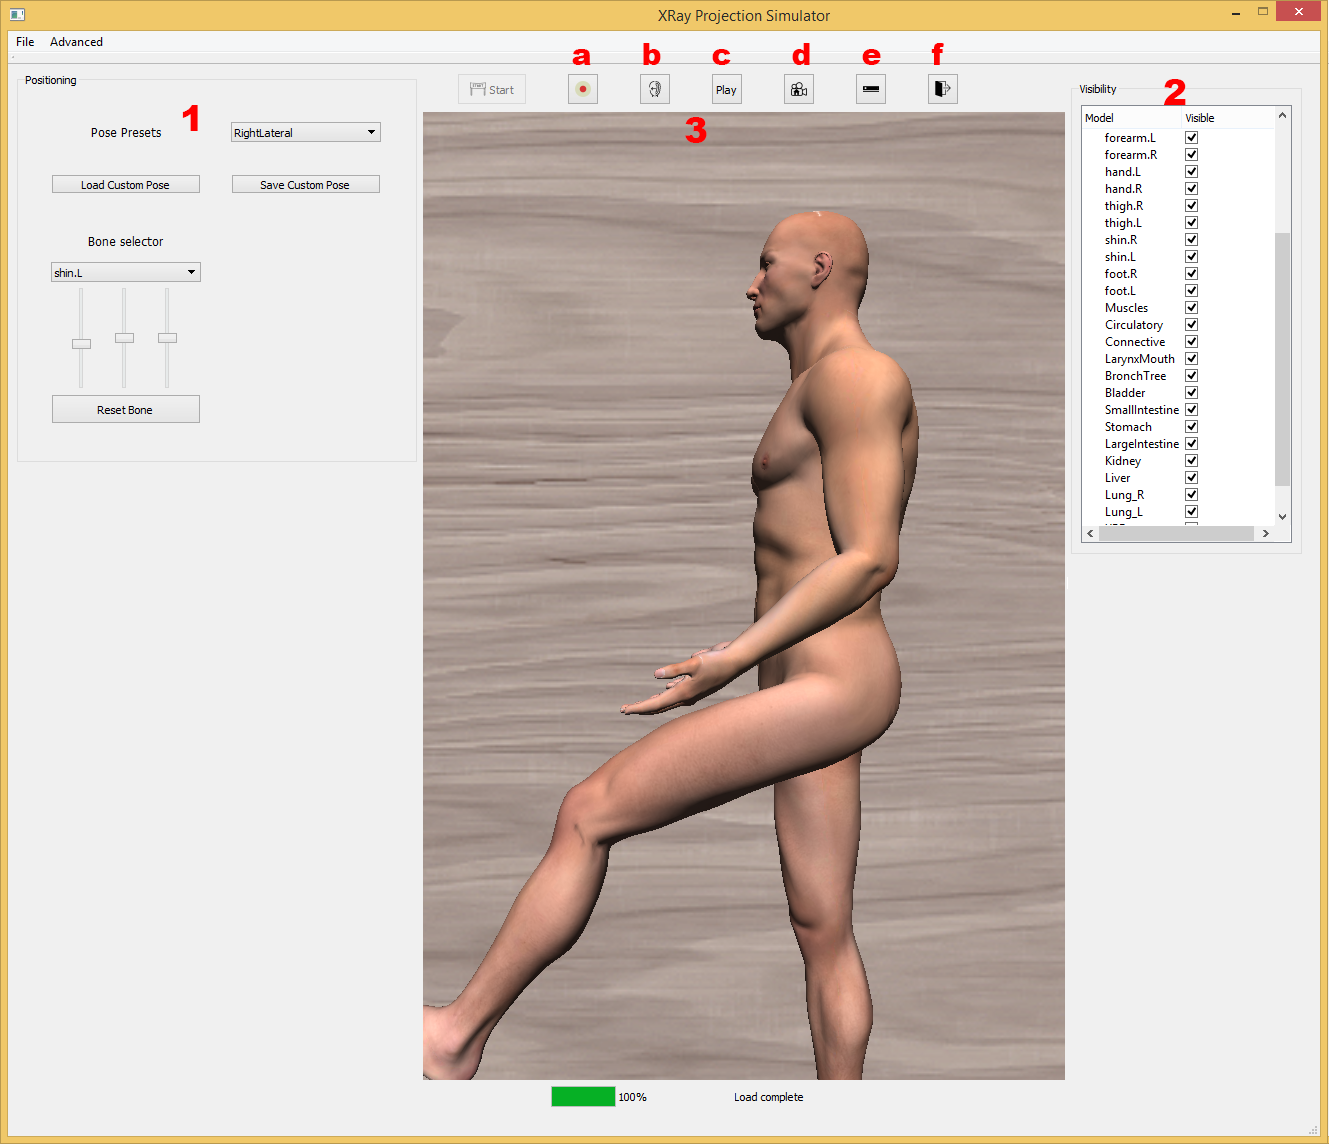
\includegraphics[width=0.9\textwidth]{IMG/posingui.png}
    \caption{Interfaz de usuario de \acs{TPTVPH} para la realización de poses. 1: Interfaz para modificar la postura del paciente virtual. 2: Lista de todos los modelos anatómicos que contenga el paciente virtual. 3: Ventana que muestra la escena virtual y en la barra superior se encuentran botones auxiliares.}
    \label{fig:posui}
\end{figure}



\section{Integración en  ITGVPH}
\label{rasim:herramienta}

%La herramienta \ac{ITGVPH} nace con el objetivo de conseguir una base de datos extensa de pacientes virtuales medios que representen una gran variabilidad anatómica. Además, permite transformar estos modelos de pacientes virtuales usando un conjunto de poses guardadas con anterioridad. %Estas poses tienen que ser generadas por un profesional cualificado a través de una interfaz de usuario, que permita al supervisor realizar cuantas posiciones se necesiten para distintos modelos anatómicos diferentes. 

Dentro del proyecto \ac{RASimAs}, el \acs{WP} 3 define todas las tareas que son necesarias para la creación de la \emph{suite} \ac{ITGVPH}, donde la tarea 3.6 se encarga de la integración
del resto de tareas. El equipo de \ac{FORTH} ha liderado el proceso de integración de todas las tareas que contó con la colaboración activa del autor de esta tesis.



% El principal objetivo es la interconexión de las etapas para conseguir la automatización de la herramienta. Por ello, los diferentes resultados producidos por cada tarea tienen que ser recogidos por esta herramienta para generar pacientes virtuales que serán utilizables tanto por el simulador \ac{RASim}. La herramienta será la encargada de las diferentes etapas para construir \ac{VPH}, desde la adquisición y procesamiento de las imágenes médicas (\ac{TC}, \ac{IRM}, etc...), el enriquecimiento el \ac{VPH} con ayuda de modelos \emph{ZygoteBody}$^{TM}$\cite{kelc2012zygote}, la adaptación del modelo de una postura a otra y la generación de las representaciones visuales y mecánicas necesarias que se utilizan finalmente en \ac{RASim}. Todas estas tareas han sido diseñadas para que puedan ser enlazadas unas con otras compartiendo el formato en su entrada y salida para automatizar la herramienta y eliminar la necesidad de tener conocimientos técnicos para poder completar todo el cauce. 
% La salida de \ac{ITGVPH} consiste en una representación superficial y volumétrica que será utilizada en el entorno de entrenamiento.




% \subsection{Caso de uso}
% \label{rasim:casodeuso}
% A continuación, se va a describir el caso de uso de la herramienta \ac{ITGVPH} que permite crear un \ac{VPH}.

% En este escenario, un usuario (profesional sanitario) puede iniciar el proceso seleccionando las imágenes médicas almacenadas en una base de datos. Estos datos suelen estar agrupados por región anatómica y existen variedad entre ellos. A continuación, el usuario podrá seleccionar los parámetros biomecánicos que se incorporarán en el modelo final, y a partir de aquí, la herramienta \ac{ITGVPH} toma el control y lanza las etapas de la herramienta con los datos de entrada seleccionados. Si se requiere, la herramienta \ac{TPTVPH} mostrará una interfaz de usuario por si es necesario modificar la postura del \ac{VPH}, pero puede elegirse una configuración anteriormente definida. En la sección anterior se ha descrito el desarrollo de la herramienta \ac{TPTVPH} que permite la adaptación del modelo anatómico.
% La salida de la herramienta consiste en dos archivos que contienen la representación superficial y volumétrica (en formato \ac{X3D} y \ac{VTU} respectivamente) del modelo generado. Estos ficheros están preparados para utilizarse en el entorno de entrenamiento utilizando \ac{RASim}.

%el usuario inicia el proceso seleccionando un conjunto de imágenes médicas que provienen de una base de datos. Estos datos suelen estar agrupados por región anatómica y existen variedad entre ellos. A continuación, el usuario puede definir o cargar un fichero dónde se encuentren los parámetros biomecánicos que se vayan a utilizar en los tejidos de la región seleccionada. El usuario puede seleccionar también si quiere alguna pose predefinida o quiere realizarla por sí mismo en una ventana interactiva. A partir de entonces, la herramienta toma el control y lanza las etapas de la herramienta con los datos de entrada seleccionados. La salida de la herramienta consiste en dos archivos que contienen la representación superficial y volumétrica (en formato \ac{X3D} y \ac{VTU} respectivamente) del modelo generado. Estos ficheros están preparados para utilizarse en el entorno de entrenamiento utilizando \ac{RASim}.

%De esta manera, un usuario (un profesional sanitario) puede iniciar el proceso seleccionando las imágenes médicas almacenadas en una base de datos. A continuación, el usuario podrá seleccionar los parámetros biomecánicos que se incorporarán en el modelo final, y a partir de aquí, la herramienta \ac{ITGVPH} toma el control, donde suministra y recoge los datos necesarios de cada etapa. Si se requiere, la herramienta \ac{TPTVPH} mostrará una interfaz de usuario por si es necesario modificar la postura del \ac{VPH}, pero puede elegirse una configuración anteriormente definida. En la sección anterior se ha descrito el desarrollo de la herramienta \ac{TPTVPH} que permite la adaptación del modelo anatómico.

%\subsection{Arquitectura lógica}
%\label{rasim:arq}

En las etapas iniciales del proyecto \ac{RASimAs} se establecieron las condiciones que tiene que cumplir la integración final:
\begin{itemize}
    \item Cada etapa no debe ser consciente de la existencia de las otras y trabajarán de manera autónoma e independiente.
    
    \item El usuario solo interactuará con una única aplicación en vez de tratar con cada proceso por separado, resultando de mayor facilidad para un usuario sin conocimientos técnicos. La interacción se limitará a seleccionar los parámetros de entrada y a la selección de pose de manera interactiva en el módulo de posicionamiento.
    
    \item La herramienta tendrá un comportamiento modular. Algunas de las tareas podrán ser omitidas si su ejecución no es necesaria. Por ejemplo, la tarea del registro no es necesaria si lo que se pretende es solo reposicionar el mismo modelo generado con anterioridad a otra postura requerida.
    
    \item El diseño permitirá la renovación o introducción de nuevas etapas en el futuro. Además, se podrán actualizar técnicas que se utilizan en los procesos, paralelizar procesos que no sean dependientes o introducir nuevas necesidades en la herramienta.
\end{itemize}

En la figura \ref{fig:toolarq} se muestra la arquitectura diseñada para la herramienta \ac{ITGVPH}.  Está compuesta por tres tareas que se han desarrollado dentro del contexto del proyecto \ac{RASimAs} e integradas en una herramienta para hacerla semi-automática. Los módulos son los siguientes: 
\begin{itemize}
    \item Módulo de registro:
    genera el modelo superficial en formato \ac{X3D} en base a un modelo anatómico de referencia y una imagen médica procedente de una base de datos. Este módulo ha sido desarrollado por \ac{UKA-IMI}, correspondiente a las tareas 3.1 y 3.2.
    \item Posicionamiento (\ac{TPTVPH}):
    se procede a reposicionar el \ac{VPH} a la posición seleccionada por el usuario al configurar la herramienta. Este módulo ha sido desarrollado por el autor de esta tesis, adaptando el método propuesto al cauce de la herramienta. Este paso corresponde a la tarea 3.5.
    \item Generación del modelo volumétrico:
    se generan los modelos mecánicos que se utilizarán en la simulación física del simulador. Este módulo ha sido desarrollado por \ac{INRIA}, correspondiendo a la tarea 3.3.
\end{itemize}

\begin{figure}
    \centering
    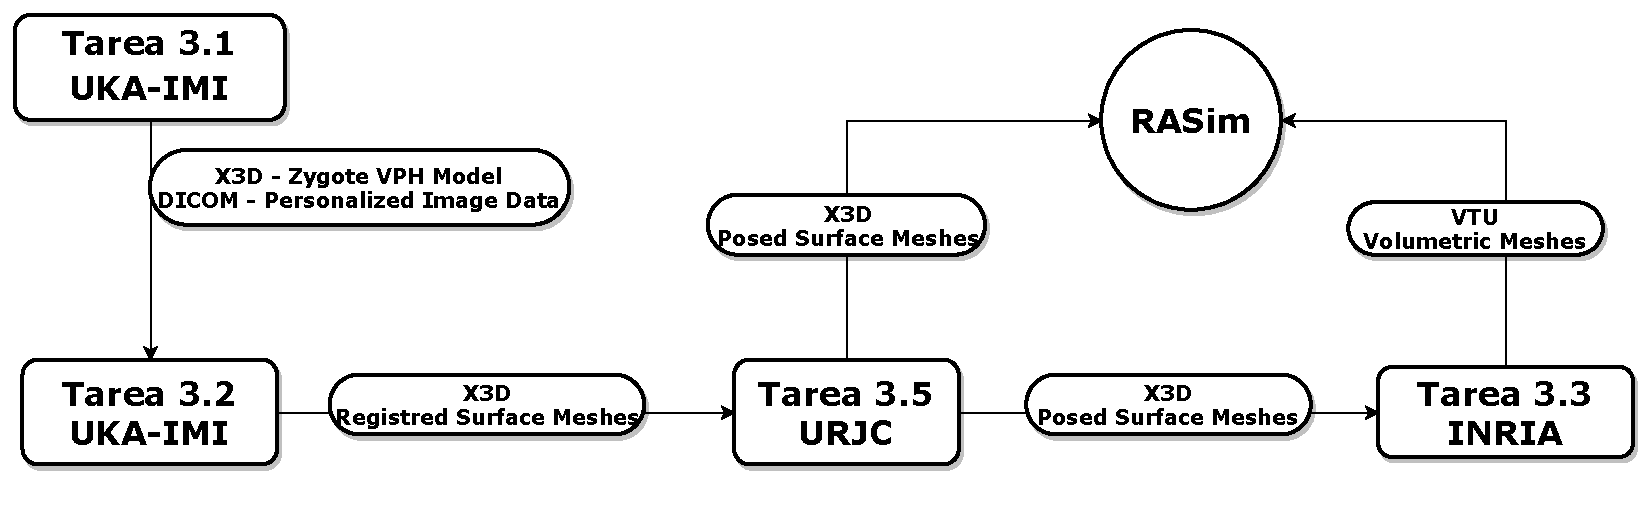
\includegraphics[width=1\textwidth]{IMG/DiagramaITGVPH.pdf}
    \caption{Arquitectura propuesta para la herramienta \acs{ITGVPH}. El formato de intercambio es \acs{X3D} y \acs{VTU}.}
    \label{fig:toolarq}
\end{figure}

Hay que destacar que no se integró  la tarea 3.4 (enumerada en la sección \ref{art:rasimas}) que se encargaba de la generación de la descripción fisiológica al no ser necesaria. Por parte de los socios médicos del proyecto, se decidió no incluir la simulación de la técnica de estimulación eléctrica del nervio en el simulador \ac{RASim} con el objetivo de  fomentar solo la práctica de la \ac{RA} guiada por \ac{US}.

El proceso comienza con el módulo de registro diseñado por \ac{UKA-IMI}. Se procede a cargar una imagen médica que contiene la anatomía objetivo, procedente de una base de datos que almacena diferentes imágenes médicas (el formato escogido es llamado \acs{DICOM}), además del modelo superficial anatómico de referencia en formato \ac{X3D}. Después, se realiza un registro automático entre la imagen médica y el modelo comercial, dando como resultado un nuevo modelo que será el primer paso para crear un \ac{VPH}. Para más información se puede consultar \cite{deOliveira:2015}. Este resultado será la entrada de la siguiente etapa.

En la segunda etapa se utiliza el módulo de posicionamiento. Esta etapa se corresponde al objetivo principal de esta tesis ampliamente descrito en el capítulo \ref{cap:posing}. Este recibe el modelo \ac{VPH} que contiene el modelo superficial y la anatomía interna, permitiendo a los usuarios seleccionar y generar posiciones útiles para el entrenamiento.

Finalmente, el modelo superficial resultante es suministrado al último módulo desarrollado por \ac{INRIA}. Esta tarea se encarga de generar el modelo volumétrico con  información biomecánica.
Tanto el modelo resultante superficial como el modelo volumétrico producidos por la herramienta \ac{ITGVPH}, se utilizarán por el simulador \ac{RASim}. Para más información se puede consultar \cite{ded3.3}.



%A continuación, se va a proceder a explicar cada etapa por separado.


% \subsubsection{Generación del modelo anatómico}
% Este módulo ha sido desarrollado por \ac{UKA-IMI} con el objetivo de realizar un registro entre las imágenes médicas y el modelo anatómico de referencia. Como se puede observar en la figura \ref{fig:r32}, el módulo ha sido divido en 5 tareas:
% %Deliverable D3.22:
% \begin{figure}[h]
%     \centering
%     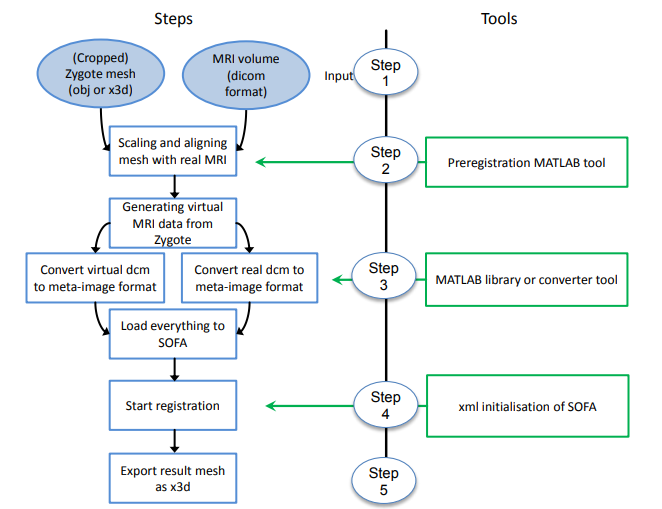
\includegraphics[width=0.5\textwidth]{IMG/rasimasd32.PNG}
%     \caption{ Diagrama de flujo de la herramienta de generación de modelo anatómico}
%     \label{fig:r32}
% \end{figure}
% \begin{enumerate}
%     \item  Se seleccionan los modelos de entrada (p. ej. \emph{ZygoteBody}$^{TM}$) e imágenes médicas (p. ej. \ac{IRM}) con los que se va a trabajar. Se procede a realizar un primer descarte de las estructuras anatómicas que se encuentran fuera de la región de interés de las imágenes médicas (por ejemplo, se eliminan brazos, cabeza, etc. si se va a trabajar sólo con la cadera).
%     \item Registro grueso: se procede a posicionar el modelo anatómico y las imágenes médicas en el mismo sistema de coordenadas y se crea el primer alineamiento (pre-registro) para prepararlo para el registro fino más adelante. Se procede a realizar un registro grueso utilizando \cite{antoinemri}. Esta técnica genera una imagen médica reconstruida para las dos representaciones e intenta ajustarlas para conseguir una alineación en cuanto a translación, rotación y escalado.
%     \item Conversión de formatos: se procede a convertir ambos modelos a una imagen 3D que es capaz de leer el software \ac{SOFA}, que será el encargado de realizar la siguiente etapa.
%     \item Registro fino: utilizando la técnica desarrollada en \cite{gilles2008}, se realiza un registro que permite deformaciones plásticas y elásticas entre dos modelos.
%     \item Por último, el modelo final se convierte al formato de intercambio para la herramienta.
% \end{enumerate}

% %%%%%%%%%%%%%%%%%%
% \subsubsection{Posicionamiento del paciente}
% Esta herramienta ya ha sido ampliamente descrita en la sección \ref{rasim:posing}. 
% No obstante, ha sido necesario realizar unas modificaciones adicionales para poder incorporar el algoritmo propuesto, a esta herramienta.


% \subsubsection{Generación del modelo volumétrico}

% Este módulo tiene como objetivo generar una malla volumétrica con los parámetros biomecánicos usados por el simulador \ac{RASim}. Desarrollado por \ac{INRIA}, se componen de los siguientes pasos:
% \begin{enumerate}
%     \item Se crea una imagen 3D basada en \emph{vóxeles} al igual que el proceso de volumetrización explicado en la sección \ref{posing:volumetrizacion}. Se etiqueta cada \emph{vóxel} con el tejido al que corresponde y así poder generar una imagen volumétrica que contenga todos los tejidos.
% \item En esta etapa se genera una malla de tetraedros a partir de la imagen 3D de la etapa anterior. Para ello, se utiliza la librería \ac{CGAL}.
% Para cada dominio (todos aquellos \emph{vóxeles} con la misma etiqueta) el algoritmo determina un conjunto optimizado de tetraedros que cumpla con los parámetros (ver anexo \ref{anexo:criterios}).  
% La malla generada es exportada al formato \ac{VTU} que contendrá toda la información necesaria para la simulación.
% Además, se incorpora información adicional que permita al núcleo de simulación calcular ciertos comportamientos. Por ejemplo, los vértices que están en contacto con un tejido óseo son marcados para que en el simulador \ac{RASim} pueda interpretarlos y generar una respuesta háptica al módulo de inserción de aguja.

% \end{enumerate}

Es importante destacar que, aunque las tres etapas crean modelos volumétricos del mismo modelo anatómico, la finalidad de cada uno es diferente y los parámetros difieren según el objetivo de este, por lo que no pueden ser compartidos. El detalle y las dimensiones que se consiguen en el módulo de posicionamiento \ac{TPTVPH} son muy superiores a las recomendadas como salida de la tercera etapa, ya que no se van a ejecutar simulaciones físicas sobre esa malla. Además, también se tiene en cuenta el objetivo de que las tareas puedan ser omitidas individualmente y tratadas como cajas negras para no compartir nada más que los datos necesarios para llegar al resultado final.



% \subsection{Interfaz de usuario}
% \label{rasim:herramientaui}

\begin{figure}[htbp]
    \centering
    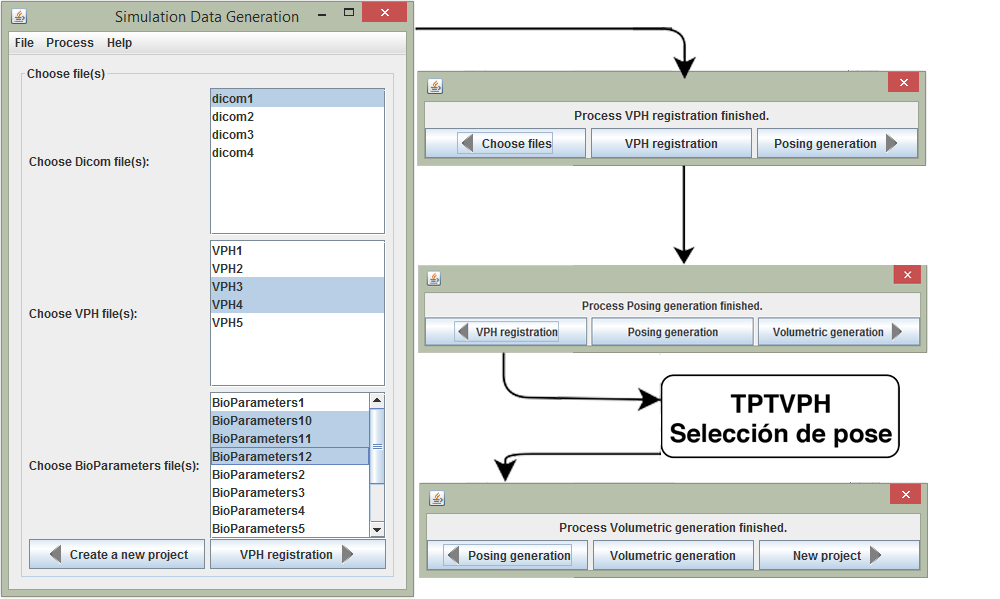
\includegraphics[width=0.8\textwidth]{IMG/toolkitui.png}
    \caption{Interfaz de la herramienta \acs{ITGVPH}. El usuario elegirá los modelos con los que quiere trabajar. Avanzará en el proceso hasta que la herramienta \acs{TPTVPH} le pregunte por la selección de pose. Una vez terminado, la herramienta sigue con el proceso.}
    \label{fig:toolui}
\end{figure}


%A continuación, se muestra la interfaz desarrollada para la herramienta \ac{ITGVPH}.
La interfaz ha sido diseñada para tener la mínima complejidad, debido a que se pretende reducir la dificultad para usuarios sin perfil técnico. De esta manera, la interfaz de la herramienta se puede resumir en la figura \ref{fig:toolui}. En esta figura se puede observar que en la primera ventana se pueden seleccionar todos los parámetros necesarios para que la herramienta trabaje de forma automática.
En orden, el primer parámetro que se puede seleccionar es el conjunto de imágenes médicas que están disponibles. Como se muestra en la figura, en este caso se disponen de imágenes en formato \acs{DICOM}.
Seguidamente, el segundo parámetro es el modelo anatómico de referencia que se pretende usar, como puede ser \emph{ZygoteBody}$^{TM}$ o \emph{Anatomium}. En los primeros prototipos sólo se ha utilizado el modelo anatómico \emph{ZygoteBody}$^{TM}$ pero la herramienta está diseñada para permitir la entrada de cualquier modelo anatómico de referencia. Este modelo será usado para hacer un registro con las imágenes anteriormente seleccionadas. 
Finalmente, se selecciona el archivo que contiene los parámetros biomecánicos y que se utilizarán en la última etapa.



Una vez están los ficheros seleccionados, el usuario sólo tendrá que avanzar a través de los menús contextuales para seguir avanzando en el proceso. Después de la fase de registro y generación del \ac{VPH}, se lanzará la interfaz de la herramienta \ac{TPTVPH} para que el usuario seleccione la postura del modelo anatómico. Una vez guardada, la herramienta seguirá con la siguiente tarea.


